% Chapters/02-Method.tex

\chapter{Methods}
\label{cp:methods}

\section{Search Strategy}

A comprehensive systematic review following \gls{prisma} guidelines was conducted between December 2023 and February 2024. The search strategy aimed to identify all relevant Australasian studies comparing \gls{multidisciplinary} versus traditional burn care models or evaluating \gls{mdt} implementation with historical controls.

\subsection{Database Search}

Primary databases searched included PubMed/MEDLINE (2014-2025), CINAHL Complete (2014-2025), Cochrane Library including Cochrane Database of Systematic Reviews, EMBASE (2014-2025), and the \gls{branz} publications database. Secondary sources included Australian Indigenous HealthInfoNet, Google Scholar (first 200 results), reference lists of included studies, \gls{anzba} conference proceedings, and institutional repositories of major burn centers.

Search terms were combined using Boolean operators:
\begin{itemize}
    \item Population: (burn* OR ``thermal injury'' OR scald*) AND (Australia* OR ``New Zealand'' OR ANZBA OR BRANZ)
    \item Intervention: (multidisciplinary OR interdisciplinary OR ``team-based'' OR ``coordinated care'' OR ``collaborative management'')
    \item Comparison: (traditional OR ``single discipline'' OR sequential OR ``usual care'')
    \item Outcomes: (mortality OR survival OR ``length of stay'' OR function* OR ``quality of life'' OR recovery)
\end{itemize}

\section{Selection Process}

Two independent reviewers screened titles and abstracts against predetermined criteria, with full-text review for potentially eligible studies. Disagreements were resolved through discussion or third reviewer consultation.

\subsection{Inclusion Criteria}
\begin{enumerate}
    \item Studies from Australasian \glspl{burnunit} published January 2014 to February 2025
    \item Adult and/or pediatric burn populations with acute injuries
    \item Evaluation of \gls{multidisciplinary} models or team-based interventions
    \item Clinical outcomes including mortality, length of stay, complications, functional measures, or \gls{qol}
    \item Quantitative or qualitative research designs
    \item English language publication
\end{enumerate}

\subsection{Exclusion Criteria}
\begin{enumerate}
    \item Non-Australasian settings
    \item Case reports with fewer than 10 patients
    \item Opinion pieces without empirical data
    \item Conference abstracts without full publication
    \item Studies exclusively examining chronic burn reconstruction
    \item Animal or laboratory studies
\end{enumerate}

\section{Data Extraction and Quality Assessment}

Standardized data extraction captured study characteristics, population details, intervention descriptions, outcome measures, and results. Quality assessment employed Oxford Centre for Evidence-Based Medicine criteria, evaluating study design, risk of bias, sample size, outcome measurement, and statistical analysis appropriateness.

\section{PRISMA Flow Diagram}

\begin{figure}[htbp]
    \centering
    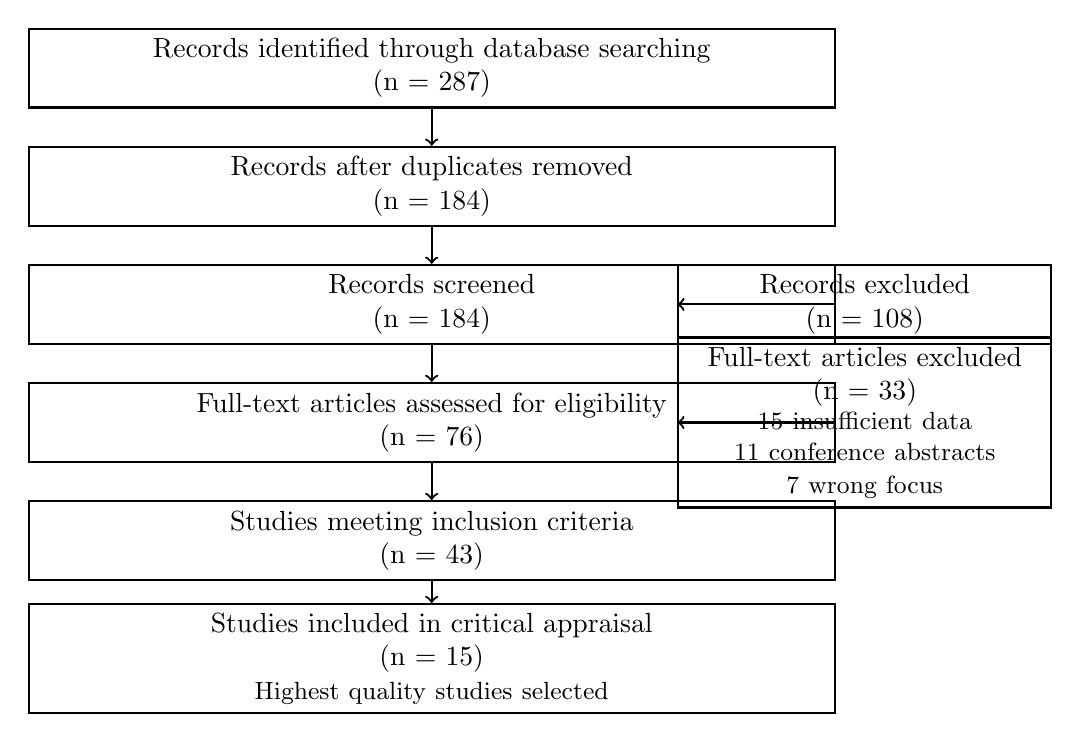
\begin{tikzpicture}[node distance=1.5cm, auto,
        box/.style={rectangle, draw=black, thick, text width=10cm, minimum height=1cm, align=center},
        smallbox/.style={rectangle, draw=black, thick, text width=4.5cm, minimum height=1cm, align=center}]
        
        % Identification
        \node[box] (identification) {Records identified through database searching\\(n = 287)};
        
        % After duplicates
        \node[box, below of=identification] (afterdup) {Records after duplicates removed\\(n = 184)};
        
        % Screening
        \node[box, below of=afterdup] (screened) {Records screened\\(n = 184)};
        \node[smallbox, right of=screened, xshift=4cm] (excluded1) {Records excluded\\(n = 108)};
        
        % Full-text assessment
        \node[box, below of=screened] (fulltext) {Full-text articles assessed for eligibility\\(n = 76)};
        \node[smallbox, right of=fulltext, xshift=4cm] (excluded2) {Full-text articles excluded\\(n = 33)\\\small{15 insufficient data\\11 conference abstracts\\7 wrong focus}};
        
        % Included studies
        \node[box, below of=fulltext] (included) {Studies meeting inclusion criteria\\(n = 43)};
        
        % Final synthesis
        \node[box, below of=included] (synthesis) {Studies included in critical appraisal\\(n = 15)\\{\small Highest quality studies selected}};
        
        % Draw arrows
        \draw[thick, ->] (identification) -- (afterdup);
        \draw[thick, ->] (afterdup) -- (screened);
        \draw[thick, ->] (screened) -- (fulltext);
        \draw[thick, ->] (fulltext) -- (included);
        \draw[thick, ->] (included) -- (synthesis);
        \draw[thick, ->] (screened) -- (excluded1);
        \draw[thick, ->] (fulltext) -- (excluded2);
        
    \end{tikzpicture}
    \caption{PRISMA flow diagram showing study selection process}
    \label{fig:prisma}
\end{figure}

The systematic search identified 287 potentially relevant articles as shown in \autoref{fig:prisma}. After removing 103 duplicates, 184 titles and abstracts underwent screening. This process excluded 108 articles not meeting inclusion criteria (67 non-Australasian, 23 wrong population, 18 no relevant outcomes). Full-text assessment of 76 articles led to exclusion of 33 studies. The final analysis included 43 studies meeting all criteria, with 15 highest-quality studies selected for detailed critical appraisal bas